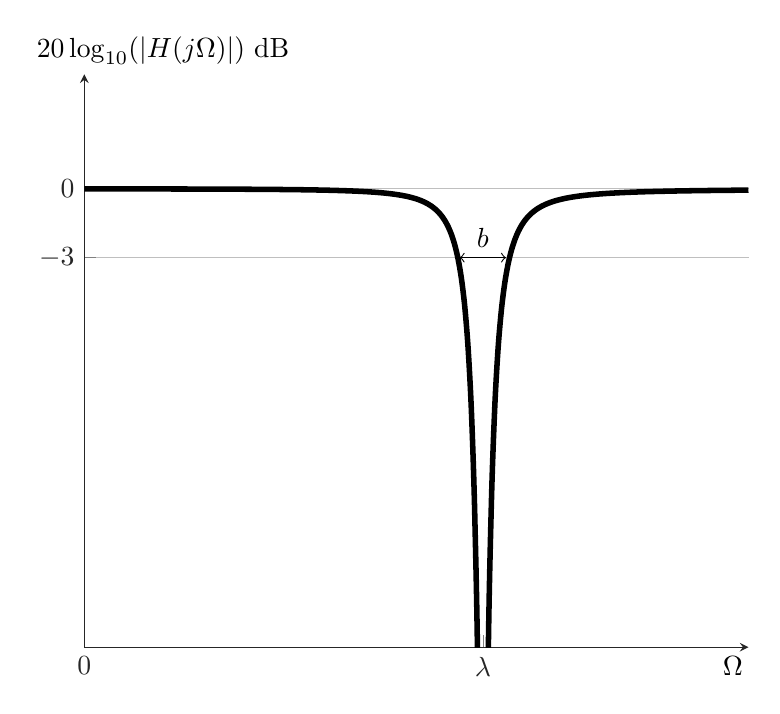
\begin{tikzpicture}
\begin{axis}[
name=plot2,
%at=(plot1.below south east), anchor=above north east, xshift=1cm,
%axis lines*=middle,
axis x line*=bottom,
axis y line*=left,
enlargelimits = false, clip=true,
scale only axis,
axis line style={->,>=stealth, shorten >= 0pt},
xlabel={$\Omega$},
ylabel={$20\log_{10}(|H(j\Omega)|)$ dB},
every axis x label/.style={
	at={(ticklabel* cs:1)},
	xshift=-0.2cm,
	anchor=north,
},
every axis y label/.style={
	at={(ticklabel* cs:1)},
	xshift=1cm,
	anchor=south,
},
every outer x axis line/.append style={white!15!black},
every x tick label/.append style={font=\color{white!15!black}},
xmin=0, xmax=100,
ymin=-20, ymax=5,
xtick={0, 60},
xticklabels={0, $\lambda$},
ytick={0, -3},
ymajorgrids,
every outer y axis line/.append style={white!15!black},
every y tick label/.append style={font=\color{white!15!black}},
legend style={draw=white!15!black,fill=white,legend cell align=left, at={(axis cs: 1.05, -5)}}]

\def\lamb{60}
\def\b{5}
\addplot [smooth, color=black, solid, line width=2pt, domain=0:100, samples=200] {20*log10((-x^2 + \lamb^2)^2/((-x^2 + \lamb^2)^2 + (\b*x)^2))};

\draw[<->] (axis cs: 56.5, -3) to (axis cs: 63.5, -3);
\node[above] at (axis cs: 60, -3) {$b$};

\end{axis}
\end{tikzpicture}